\documentclass[a4paper]{article}
\usepackage{cmap}
\usepackage[utf8]{inputenc}
\usepackage[T2A]{fontenc}
\usepackage[english,russian]{babel} 
\usepackage[left=15mm, top=15mm, right=15mm, bottom=30mm, nohead, nofoot]{geometry}
\usepackage{blindtext}  % рыба-текст
\usepackage{graphicx}  % изобржаения
\usepackage{float} % плавающие объекты
\usepackage{wrapfig}  % изобржаения
\usepackage{tikz} % графика
\usepackage{mdframed} % рамки
\usepackage{xcolor} % определение цветов
\usepackage{nicefrac} % красивые дроби
\usepackage{cancel} % сокращение
\usepackage{amsmath,amsfonts,amssymb} % математический пакет
\usepackage{hyperref}  % гиперссылки
\usepackage{fancybox,fancyhdr} % хедер и футер
\usepackage{listings} % код
\usepackage[skip=2pt]{caption} % расстояние между подписью и картинкой
\pagestyle{fancy}
\fancyhf{}
\fancyhead[L]{Лабораторная работа №6}
\fancyhead[R]{\textit{Обработка изображений}}
\fancyfoot[C]{\thepage}
\headsep=4mm
\footskip=13mm
\setlength{\parindent}{0em}
\setlength{\parsep}{0em}
\setlength{\headheight}{12pt}
\setlength{\topmargin}{-38pt}

\definecolor{urlcolor}{HTML}{3454D1}
\definecolor{linkcolor}{HTML}{3454D1}
\hypersetup{
    pdfstartview=FitH,
    linkcolor=linkcolor,
    urlcolor=urlcolor,
    colorlinks=true,
    pdftitle={Лабораторная работа №6},
    pdfauthor={Овчинников П.А.}
}

\definecolor{strings}{rgb}{0,0.6,0}
\definecolor{comments}{rgb}{0,0.3,0}
\definecolor{numbers}{rgb}{0.5,0.5,0.5}
\definecolor{keywords}{rgb}{0.09,0.61,0.95}
\definecolor{background}{rgb}{0.97,0.97,0.97}
\lstdefinestyle{codestyle}{
    backgroundcolor=\color{background},
    commentstyle=\color{comments},
    keywordstyle=\color{keywords},
    stringstyle=\color{strings},
    numberstyle=\tiny\color{numbers},
    basicstyle=\ttfamily\footnotesize,
    breakatwhitespace=false,
    breaklines=true,
    captionpos=b,
    inputencoding=utf8,
    keepspaces=true,
    numbers=left,
    numbersep=5pt,
    showspaces=false,
    showstringspaces=false,
    showtabs=false,
    tabsize=2,
    extendedchars=true,
    literate=
    {а}{{\cyra}}1
    {б}{{\cyrb}}1
    {в}{{\cyrv}}1
    {г}{{\cyrg}}1
    {д}{{\cyrd}}1
    {е}{{\cyre}}1
    {ж}{{\cyrzh}}1
    {з}{{\cyrz}}1
    {и}{{\cyri}}1
    {й}{{\cyrishrt}}1
    {к}{{\cyrk}}1
    {л}{{\cyrl}}1
    {м}{{\cyrm}}1
    {н}{{\cyrn}}1
    {о}{{\cyro}}1
    {п}{{\cyrp}}1
    {р}{{\cyrr}}1
    {с}{{\cyrs}}1
    {т}{{\cyrt}}1
    {у}{{\cyru}}1
    {ф}{{\cyrf}}1
    {х}{{\cyrh}}1
    {ц}{{\cyrc}}1
    {ч}{{\cyrch}}1
    {ш}{{\cyrsh}}1
    {щ}{{\cyrshch}}1
    {ъ}{{\cyrhrdsn}}1
    {ы}{{\cyrery}}1
    {ь}{{\cyrsftsn}}1
    {э}{{\cyrerev}}1
    {ю}{{\cyryu}}1
    {я}{{\cyrya}}1
    {А}{{\CYRA}}1
    {Б}{{\CYRB}}1
    {В}{{\CYRV}}1
    {Г}{{\CYRG}}1
    {Д}{{\CYR96}}1
    {Е}{{\CYRE}}1
    {Ж}{{\CYRZH}}1
    {З}{{\CYRZ}}1
    {И}{{\CYRI}}1
    {Й}{{\CYRISHRT}}1
    {К}{{\CYRK}}1
    {Л}{{\CYRL}}1
    {М}{{\CYRM}}1
    {Н}{{\CYRN}}1
    {О}{{\CYRO}}1
    {П}{{\CYRP}}1
    {Р}{{\CYRR}}1
    {С}{{\CYRS}}1
    {Т}{{\CYRT}}1
    {У}{{\CYRU}}1
    {Ф}{{\CYRF}}1
    {Х}{{\CYRH}}1
    {Ц}{{\CYRC}}1
    {Ч}{{\CYRCH}}1
    {Ш}{{\CYRSH}}1
    {Щ}{{\CYRSHCH}}1
    {Ъ}{{\CYRHRDSN}}1
    {Ы}{{\CYRERY}}1
    {Ь}{{\CYRSFTSN}}1
    {Э}{{\CYREREV}}1
    {Ю}{{\CYRYU}}1
    {Я}{{\CYRYA}}1
}
\lstset{style=codestyle}

\addto\captionsrussian{
  \renewcommand{\contentsname}
    {\centering Содержание}
}
\newcommand{\addsection}[1]{
    \phantomsection
    \addcontentsline{toc}{section}{#1}
    \section*{\centering #1}
}
\newcommand{\addsubsection}[1]{
    \phantomsection
    \addcontentsline{toc}{subsection}{#1}
    \subsection*{\centering #1}
}
\newcommand{\addsubsubsection}[1]{
    \phantomsection
    \addcontentsline{toc}{subsubsection}{#1}
    \subsubsection*{\centering #1}
}

\newmdenv[
    leftmargin = 0.5em,
    skipabove = 0.5em,
    skipbelow = 0.5em,
    linewidth = 1pt,
    rightline = false,
    topline = false,
    bottomline = false
]{quotebox}

\newlength{\tempheight}
\newcommand{\Let}{
\mathbin{\text{\settoheight{\tempheight}{\mathstrut}\raisebox{0.4\pgflinewidth}{
\tikz[baseline=0.5ex,line cap=round,line join=round] \draw (0,0) --++ (0.3em,0) --++ (0,2.3ex) --++ (-0.3em,0);
}}}}
\newcommand*\squared[1]{\tikz[baseline=(char.base)]{
            \node[shape=rectangle,draw,inner sep=4pt] (char) {#1};}}
\newcommand*\msquared[1]{\tikz[baseline=(char.base)]{
            \node[shape=rectangle,draw,inner sep=4pt] (char) {$\displaystyle #1$};}}
\newcommand\argmax[1]{\underset{#1}{\text{argmax}}}
\renewcommand\max[1]{\underset{#1}{\text{max}}}
\newcommand{\at}{\biggr\rvert}
\newcommand{\shiftright}[3]{\makebox[#2][r]{\makebox[#1][l]{#3}}}
\newcommand{\e}{\;\text{e}}
\let\oldint\int
\def\int{\oldint\limits}
\DeclareRobustCommand{\divby}{%
  \mathrel{\vbox{\baselineskip.65ex\lineskiplimit0pt\hbox{.}\hbox{.}\hbox{.}}}%
}

\newcommand\NB{\textbf{N\kern-0.32em\textcolor{red}{B}}}

\begin{document}
\begin{titlepage}
    \begin{center}
    \includegraphics[width=0.18\textwidth]{~/Изображения/itmo_logo.png}\\[10pt]
        Федеральное государственное автономное образовательное \\ учреждение высшего образования \\[6pt]
        САНКТ-ПЕТЕРБУРГСКИЙ НАЦИОНАЛЬНЫЙ \\ ИССЛЕДОВАТЕЛЬСКИЙ УНИВЕРСИТЕТ ИТМО \\[16pt]
        Факультет систем управления и робототехники \vfill
        Лабораторная работа №6 \\[0.5em]
        \textbf{\MakeUppercase{Обработка изображений}}
    \end{center}\vfill
    \begin{flushright}
        Студент: Овчинников П.А.\\
        Поток: ЧАСТ.МЕТ. 1.3 \\[0.5em]
        Преподаватель: Перегудин А.А.\\Пашенко А.В.
    \end{flushright}\vfill
    \begin{center}
        {\small Санкт-Петербург \\ 2024}
    \end{center}
\end{titlepage}
\setcounter{page}{2}
\tableofcontents\newpage

В этой лабораторной работе мы научимся использовать преобразование Фурье на практике для применения различных фильтров к изображениям.
% MARK: №1
\addsection{Фильтрация изображений с периодичностью}
Начнём с фильтрации изображения с периодичностью --- это такие изображения, в которых можно заметить периодические волны. Выберем 11 изображение из списка заготовленных --- вот так оно выглядит:
\begin{figure}[H]
    \centering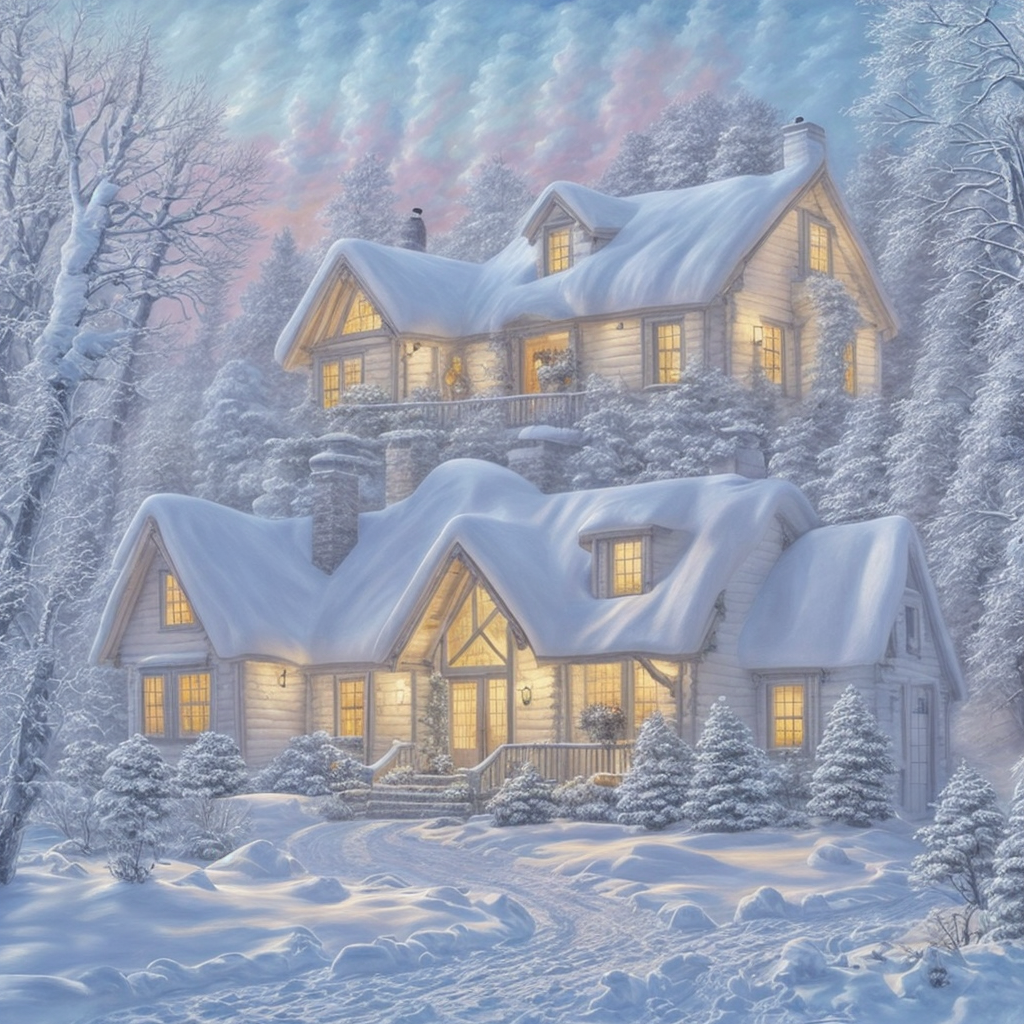
\includegraphics[width=0.35\textwidth]{sources/11.png}
    \caption{Исходное изображение}
\end{figure}
Мы видим периодически волны под углом примерно $15^\cdot$ к вертикали. Для того чтобы убрать их, нужно будет обнаружить на спектре Фурье пары симметричных пиков, которые и формируют эти волны. Для этого применим преобразование Фурье к изображению:
\begin{figure}[H]
    \hspace{5em}
    \begin{minipage}{0.35\textwidth}
        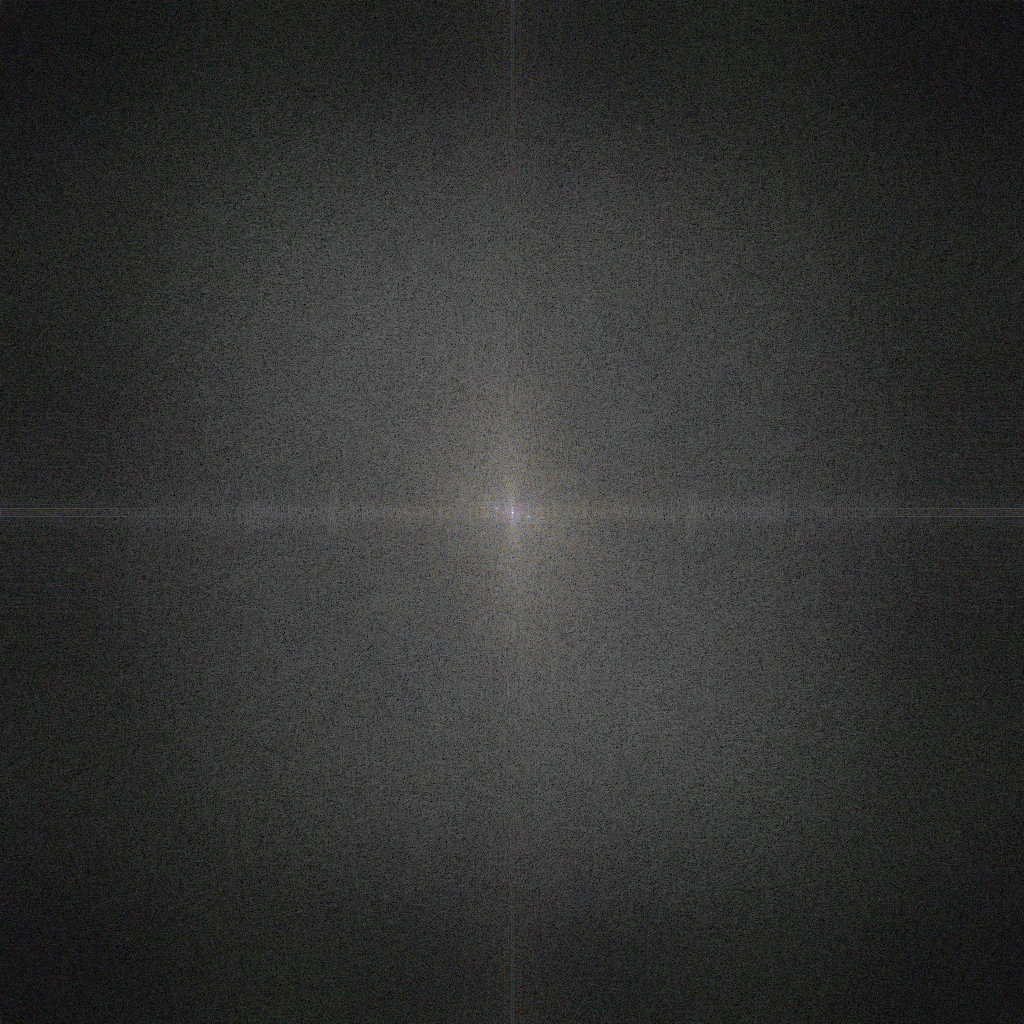
\includegraphics[width=\textwidth]{sources/1first/11_fft.png}
        \caption{Спектр Фурье}
    \end{minipage}\hfill
    \begin{minipage}{0.35\textwidth}
        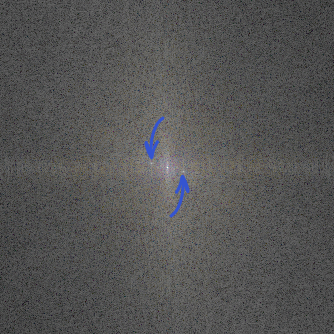
\includegraphics[width=\textwidth]{sources/1first/11_fft (scaled).png}
        \caption{Спектр Фурье (увеличенный)}
    \end{minipage}
    \hspace{5em}
\end{figure}
Изображение справа показывает в увеличении участок Фурье-образа в центре --- на нём стрелочками отмечены два симметричных пика, которые мы будем удалять. Для этого в редакторе изображений выберем умную заплатку и замажем их.\newpage
Так выглядит образ с замазанными пиками:
\begin{figure}[H]
    \centering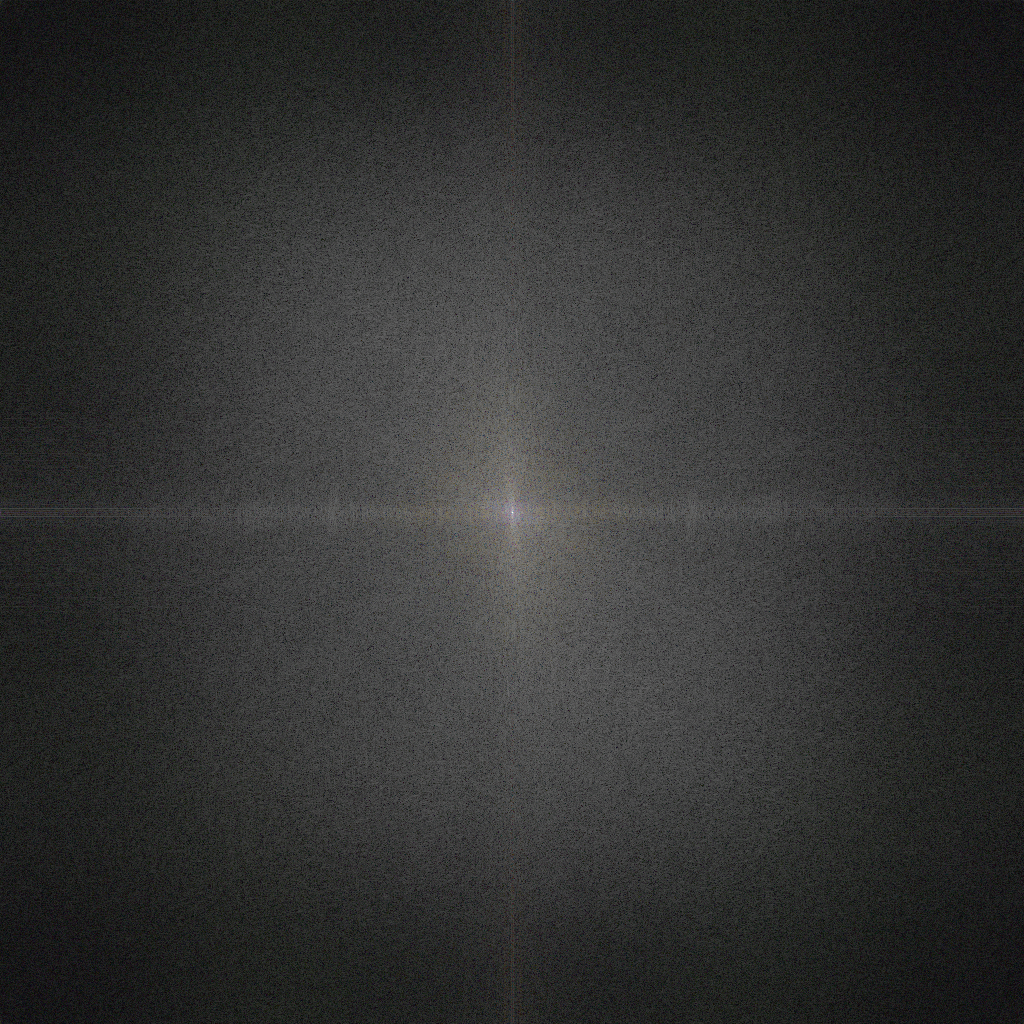
\includegraphics[width=0.35\textwidth]{sources/1first/11_fft_edited.png}
    \caption{Спектр Фурье (отфильтрованный)}
\end{figure}
Теперь применим обратное преобразование Фурье к отфильтрованному спектру и посмотрим на результат:
\begin{figure}[H]
    \centering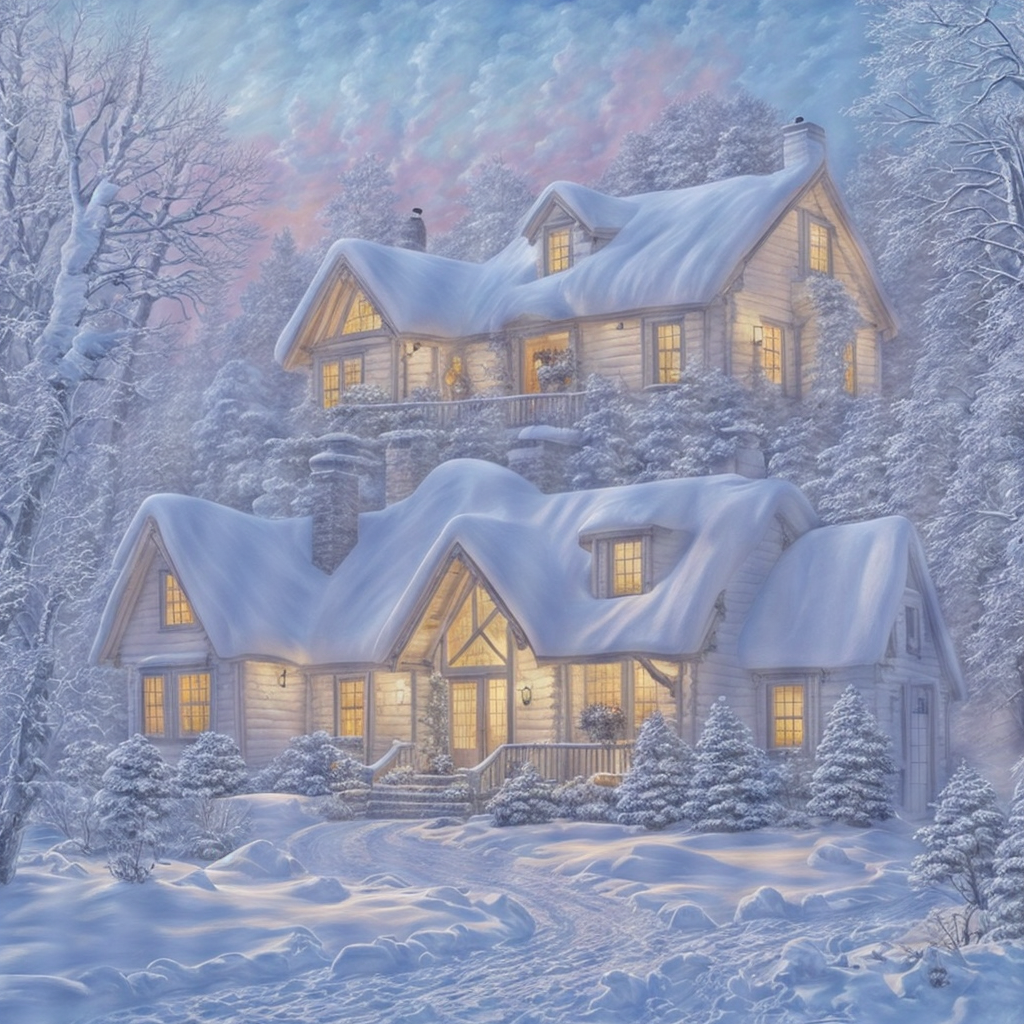
\includegraphics[width=0.35\textwidth]{sources/1first/11_filtered.png}
    \caption{Отфильтрованное изображение}
\end{figure}
Видно, что волны исчезли, и изображение стало более однородным и более «плоским». Таким образом, мы успешно отфильтровали периодичность из изображения.\newpage

% MARK: №2
\addsection{Размытие изоображения}
Перейдём к размытию изображения. Будет это делать с помощью блочного и гауссовского размытия. Возьмём вот такое изображение кота:
\begin{figure}[H]
    \centering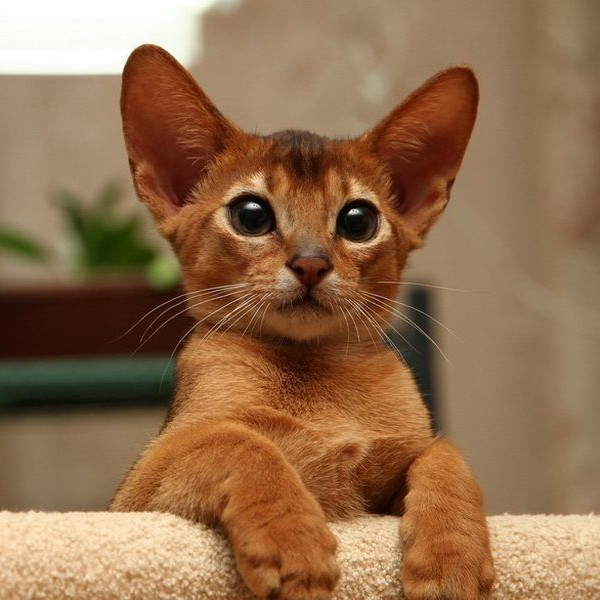
\includegraphics[width=0.35\textwidth]{sources/cat.jpg}
    \caption{Исходное изображение}
\end{figure}
Зададимся тремя нечётными значениями $n \geqslant 3$: $\left[ 9, 15, 27 \right]$. Мы будем выполнять свёртку исходного изображения с каждым из ядер фильтров --- это прямое применение фильтра. Кроме этого мы будем выполнять преобразование Фурье к изображениям и к каждому из ядер, затем перемножать их и применять обратное преобразование Фурье к результату --- это будет применение фильтра в частотной области. И сравним получившиеся результаты.
\addsubsection{Блочное размытие}
Для блочного размытия возьмём ядро следующего вида (приведён пример для $n = 3$):
$$\begin{bmatrix}
    \nicefrac{1}{9} & \nicefrac{1}{9} & \nicefrac{1}{9} \\
    \nicefrac{1}{9} & \nicefrac{1}{9} & \nicefrac{1}{9} \\
    \nicefrac{1}{9} & \nicefrac{1}{9} & \nicefrac{1}{9}
\end{bmatrix} \text{ или в общем виде матрица } n\times n \text{ вида } \begin{bmatrix}
    1 & \ldots & 1 \\
    \vdots & \ddots & \vdots \\
    1 & \ldots & 1
\end{bmatrix} \cdot \frac{1}{n^2}$$
И вот как выглядит свёртка изображения с ядром для каждого из значений $n$:
\begin{figure}[H]
    \hspace{5em}
    \begin{minipage}{0.35\textwidth}
        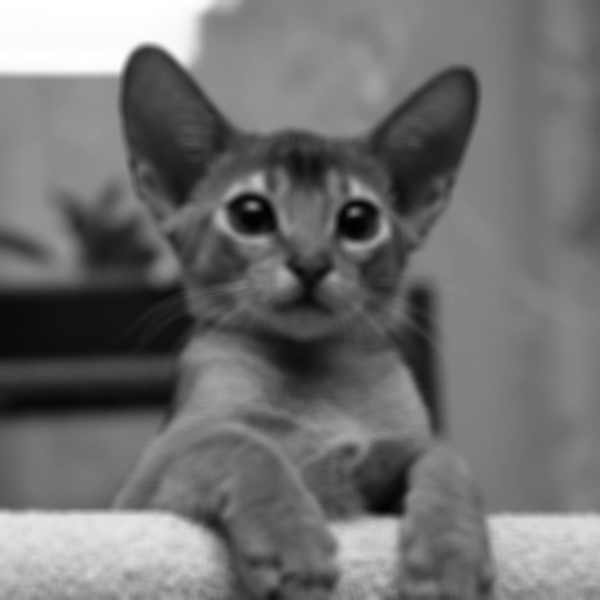
\includegraphics[width=\textwidth]{sources/2second/block_9.png}
        \caption{Блочное размытие $(n = 9)$}
    \end{minipage}\hfill
    \begin{minipage}{0.35\textwidth}
        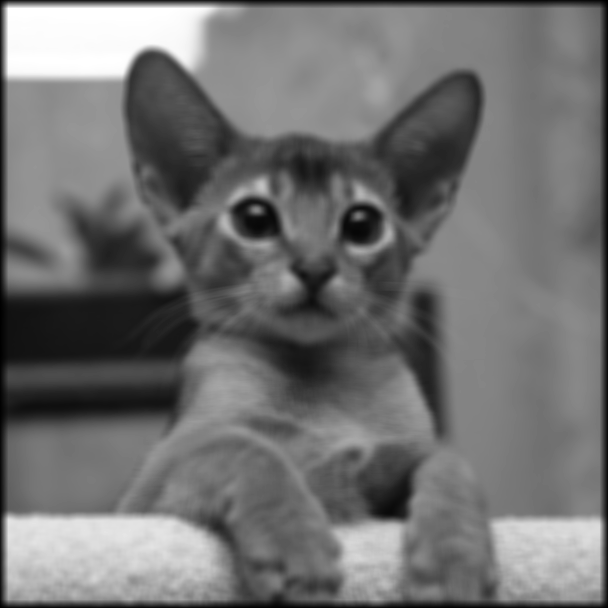
\includegraphics[width=\textwidth]{sources/2second/block_fft_9.png}
        \caption{Через Фурье-образ $(n = 9)$}
    \end{minipage}
    \hspace{5em}
\end{figure}
\begin{figure}[H]
    \hspace{5em}
    \begin{minipage}{0.35\textwidth}
        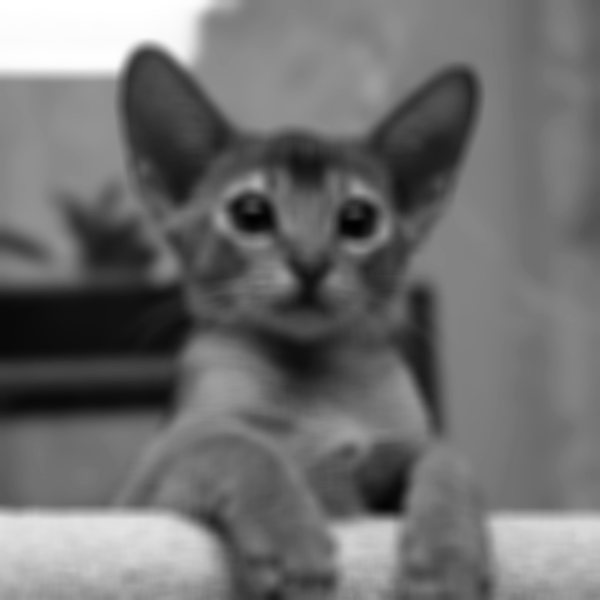
\includegraphics[width=\textwidth]{sources/2second/block_15.png}
        \caption{Блочное размытие $(n = 15)$}
    \end{minipage}\hfill
    \begin{minipage}{0.35\textwidth}
        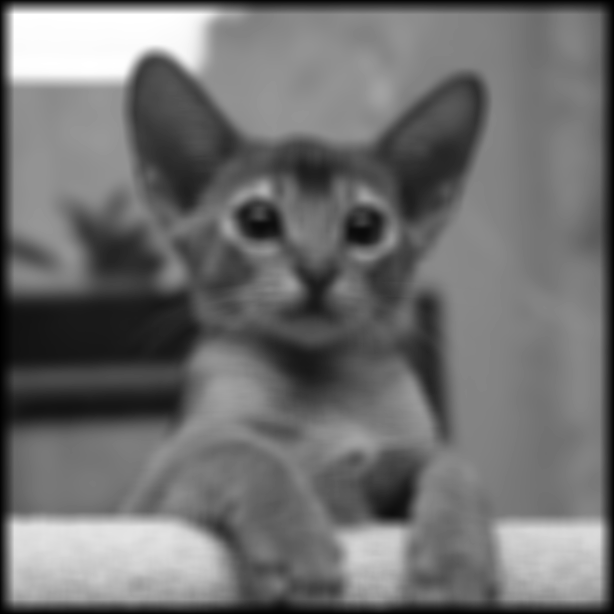
\includegraphics[width=\textwidth]{sources/2second/block_fft_15.png}
        \caption{Через Фурье-образ $(n = 15)$}
    \end{minipage}
    \hspace{5em}
\end{figure}
\begin{figure}[H]
    \hspace{5em}
    \begin{minipage}{0.35\textwidth}
        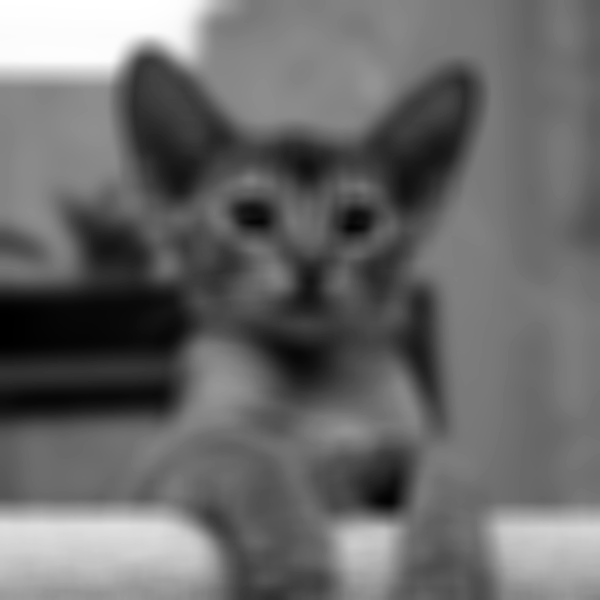
\includegraphics[width=\textwidth]{sources/2second/block_27.png}
        \caption{Блочное размытие $(n = 27)$}
    \end{minipage}\hfill
    \begin{minipage}{0.35\textwidth}
        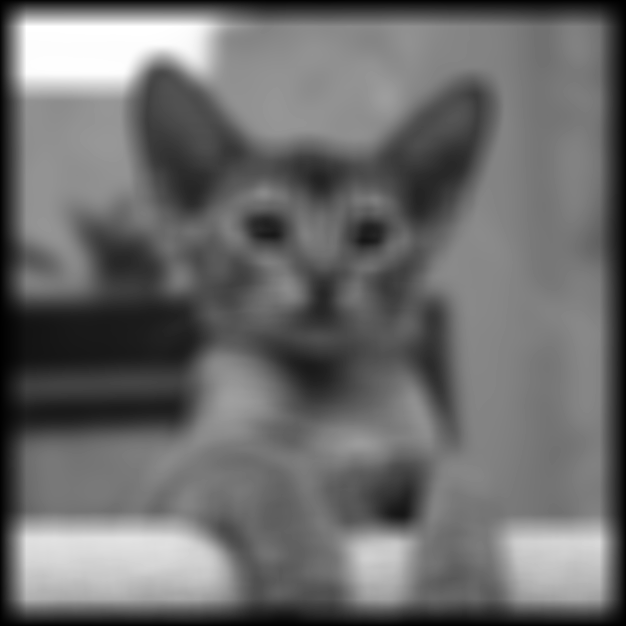
\includegraphics[width=\textwidth]{sources/2second/block_fft_27.png}
        \caption{Через Фурье-образ $(n = 27)$}
    \end{minipage}
    \hspace{5em}
\end{figure}
Как мы видим, при увеличении $n$ изображение становится всё более размытым. Применение фильтра через свёртку изображения с ядром отличается от применения фильтра через преобразование Фурье чёрной рамкой вокруг --- дело в том, что при преобразовании Фурье изображение дополняется нулями до размера, необходимо для того, чтобы применить фильтр.
\addsubsection{Гауссовское размытие}
Для гауссовского размытия возьмём ядро, которое будет заполнено значениями следующей функции:
$$f(x, y) = \e^{- \frac{9}{n^2}\left( \left( x - \frac{n + 1}{2} \right) + \left( y - \frac{n + 1}{2} \right) \right)}$$
Затем нормируем ядро так, чтобы сумма всех его элементов была равна 1 --- для этого просто поделим каждый элемент ядра на сумму всех его элементов. Вот как выглядит применение гауссовского размытия к изображению для каждого из значений $n$:

\begin{figure}[H]
    \hspace{5em}
    \begin{minipage}{0.35\textwidth}
        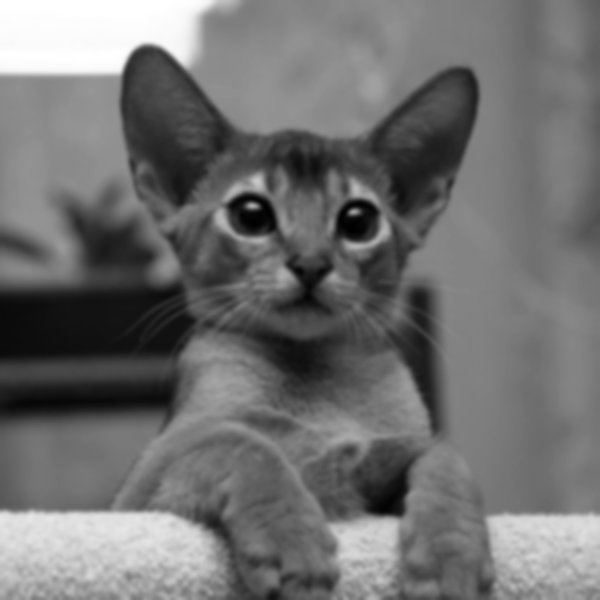
\includegraphics[width=\textwidth]{sources/2second/gauss_9.png}
        \caption{Гауссовское размытие $(n = 9)$}
    \end{minipage}\hfill
    \begin{minipage}{0.35\textwidth}
        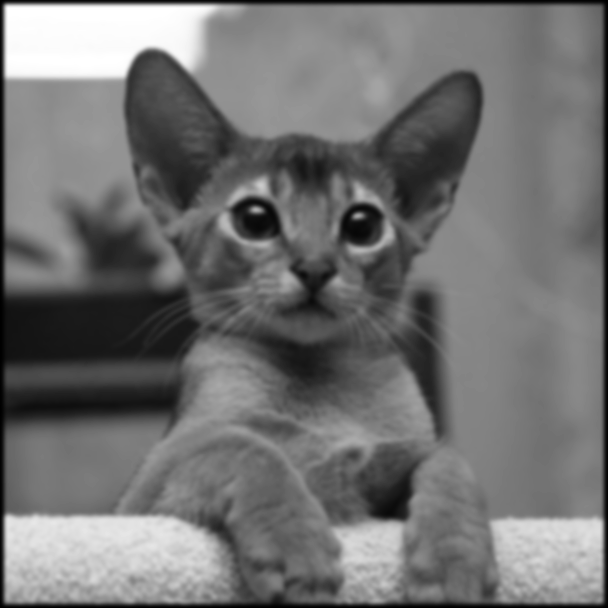
\includegraphics[width=\textwidth]{sources/2second/gauss_fft_9.png}
        \caption{Через Фурье-образ $(n = 9)$}
    \end{minipage}
    \hspace{5em}
\end{figure}
\begin{figure}[H]
    \hspace{5em}
    \begin{minipage}{0.35\textwidth}
        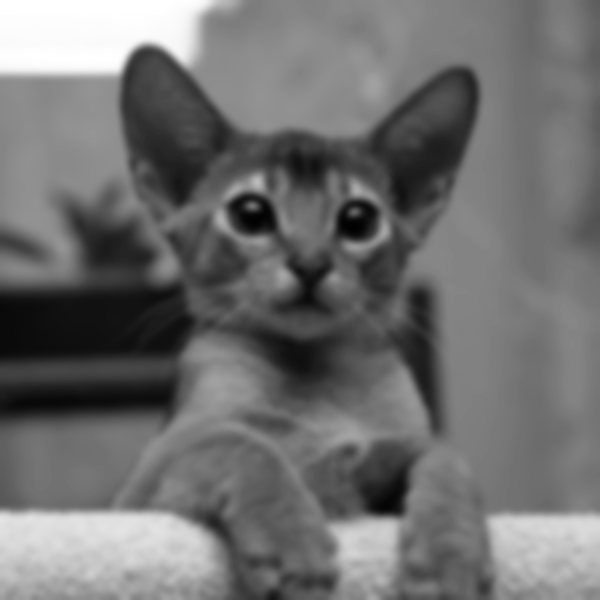
\includegraphics[width=\textwidth]{sources/2second/gauss_15.png}
        \caption{Гауссовское размытие $(n = 15)$}
    \end{minipage}\hfill
    \begin{minipage}{0.35\textwidth}
        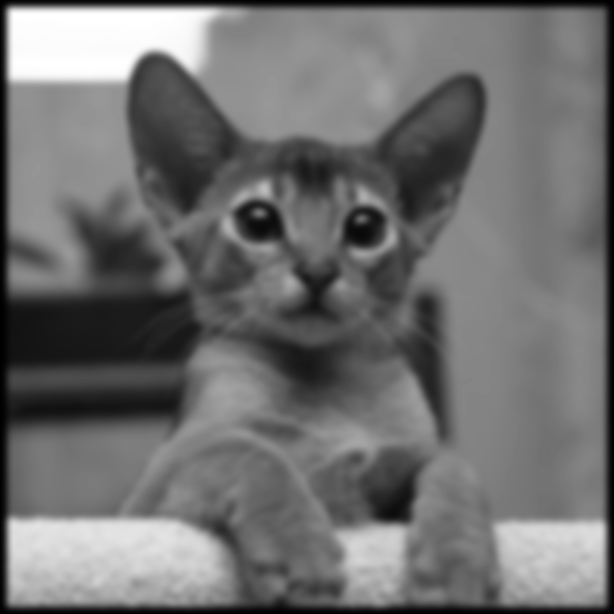
\includegraphics[width=\textwidth]{sources/2second/gauss_fft_15.png}
        \caption{Через Фурье-образ $(n = 15)$}
    \end{minipage}
    \hspace{5em}
\end{figure}
\begin{figure}[H]
    \hspace{5em}
    \begin{minipage}{0.35\textwidth}
        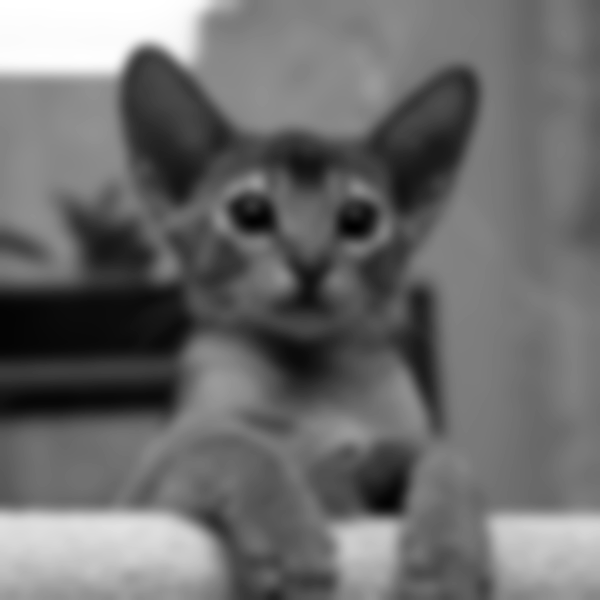
\includegraphics[width=\textwidth]{sources/2second/gauss_27.png}
        \caption{Гауссовское размытие $(n = 27)$}
    \end{minipage}\hfill
    \begin{minipage}{0.35\textwidth}
        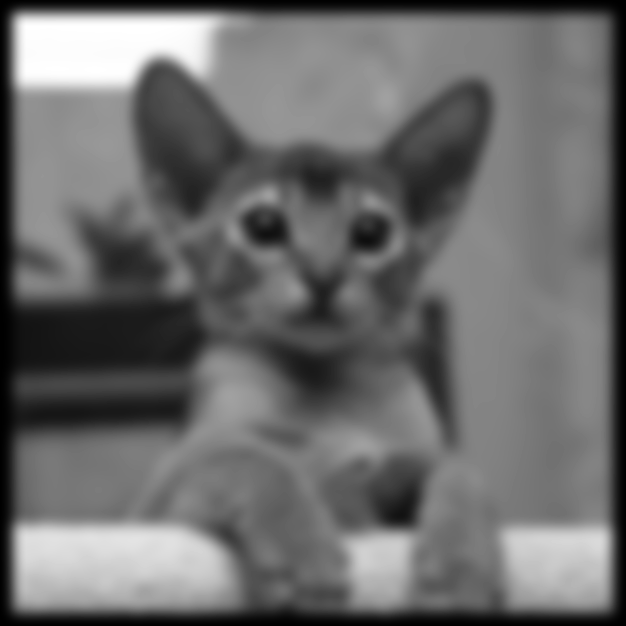
\includegraphics[width=\textwidth]{sources/2second/gauss_fft_27.png}
        \caption{Через Фурье-образ $(n = 27)$}
    \end{minipage}
    \hspace{5em}
\end{figure}
Мы видим, что в обоих случаях размытие работает одинаково хорошо, но, опять же, по выше озвученной причине у размытия через преобразования Фурье появляется чёрная рамка вокруг изображения. Если это не желательно, то лучше использовать свёртку изображения с ядром.\\[0.5em]
Теперь сравним результаты размытия изображения с помощью блочного и гауссовского фильтров. Для этого рассмотрим оба размытия путём свёртки при $n = 27$, чтобы между ними была заметна разница:
\begin{figure}[H]
    \hspace{5em}
    \begin{minipage}{0.35\textwidth}
        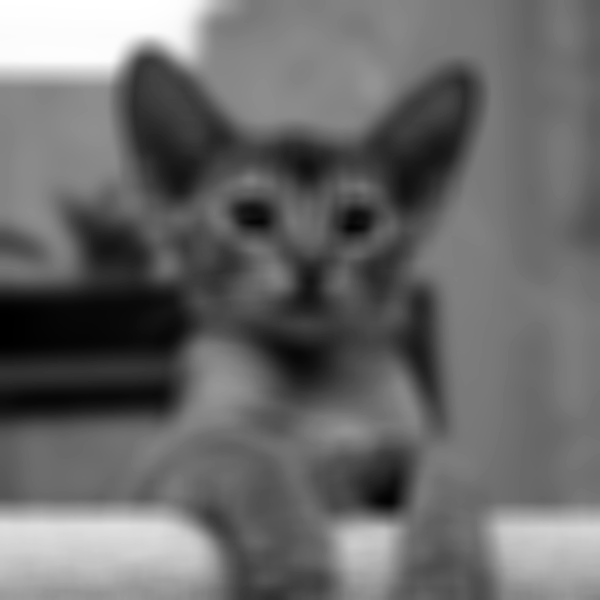
\includegraphics[width=\textwidth]{sources/2second/block_27.png}
        \caption{Блочное размытие $(n = 27)$}
    \end{minipage}\hfill
    \begin{minipage}{0.35\textwidth}
        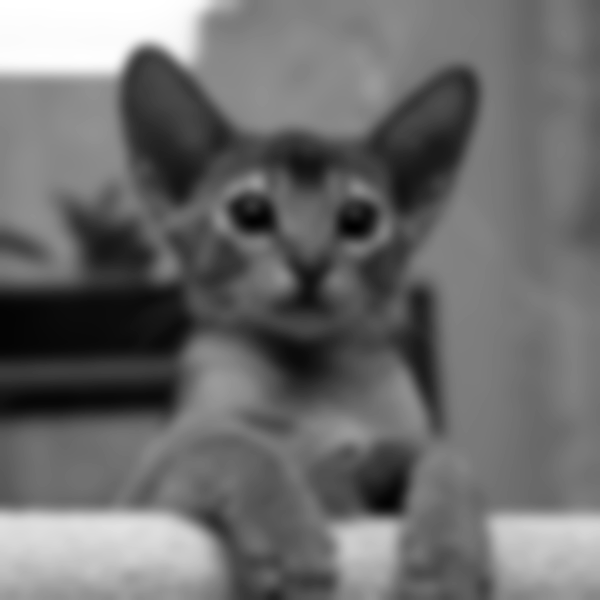
\includegraphics[width=\textwidth]{sources/2second/gauss_27.png}
        \caption{Гауссовское размытие $(n = 27)$}
    \end{minipage}
    \hspace{5em}
\end{figure}
По глазам котёнка становится очевидно, что блочное размытие больше подходит для pixel art'ов и других изображений с чёткими границами и узорами, а гауссовское размытие --- для фотографий с реальными объектами.

% MARK: №3
\addsection{Увеличение резкости}
Теперь перейдём к увеличению резкости изображения. Для этого нам понадобится ядро следующего вида:
$$\begin{bmatrix}
    0 & -1 & 0 \\
    -1 & 5 & -1 \\
    0 & -1 & 0
\end{bmatrix}$$
Найдём свёртку того же изображения кота с этим ядром. Сделаем это дважды, чтобы усилить результат --- так различия будут более заметными:
\begin{figure}[H]
    \hspace{5em}
    \begin{minipage}{0.35\textwidth}
        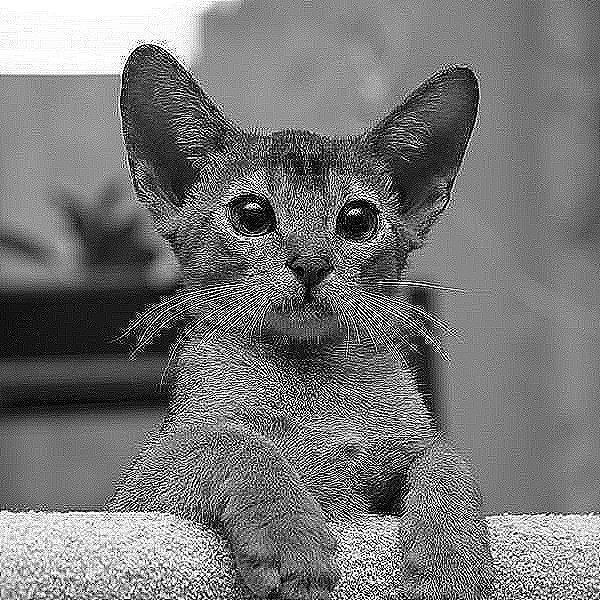
\includegraphics[width=\textwidth]{sources/3third/sharpened.png}
        \caption{Увеличение резкости}
    \end{minipage}\hfill
    \begin{minipage}{0.35\textwidth}
        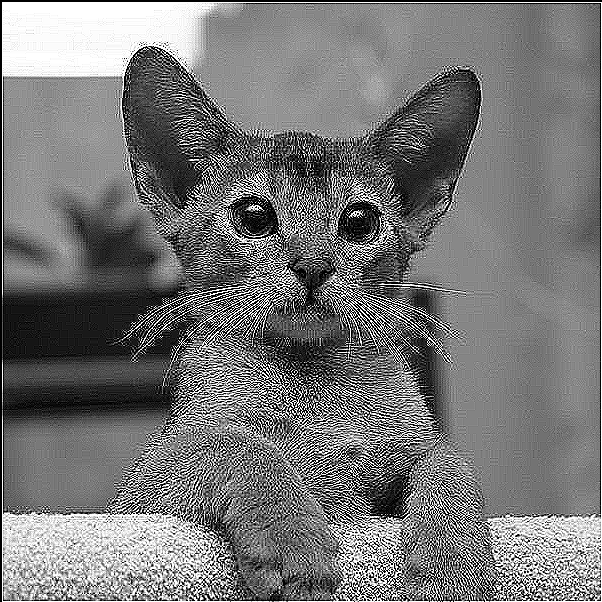
\includegraphics[width=\textwidth]{sources/3third/sharpened_fft.png}
        \caption{Через Фурье-образ}
    \end{minipage}
    \hspace{5em}
\end{figure}
Увеличение резкости действительно происходит, но вновь при применении фильтра через преобразование Фурье появляется рамка вокруг изображения, на этот раз она белого цвета. В остальном результаты одинаковы.

% MARK: №4
\addsection{Выделение краёв}
Наконец, рассмотрим выделение краёв, для которого понадобится такое ядро:
$$\begin{bmatrix}
    -1 & -1 & -1 \\
    -1 & 8 & -1 \\
    -1 & -1 & -1
\end{bmatrix}$$
Для того, чтобы проверить его работу, возьмём логотип VK на однородном фоне:
\begin{figure}[H]
    \centering
\includegraphics[width=0.6\textwidth]{sources/vk_logo.png}
    \caption{Исходное изображение}
\end{figure}
Применим к нему ядро для выделения краёв:
\begin{figure}[H]
    \hspace{4em}
    \begin{minipage}{0.4\textwidth}
        
\includegraphics[width=\textwidth]{sources/4fourth/edged.png}
        \caption{Выделение краёв}
    \end{minipage}\hfill
    \begin{minipage}{0.4\textwidth}
        
\includegraphics[width=\textwidth]{sources/4fourth/edged_fft.png}
        \caption{Через Фурье-образ}
    \end{minipage}
    \hspace{4em}
\end{figure}
И вновь мы видим, что результаты идентичны, а белая рамка вокруг изображения появляется только при применении фильтра через преобразование Фурье. В остальном всё работает как надо и в обоих случаях края выделяются.\\[2em]
\textbf{Вывод:}
\begin{quotebox}
    Мы научились сглаживать изображения с периодичнностью, пользуясь двумерным преобразованием Фурье. Также мы выяснили,     что различные фильтры можно применять не только с помощью свёртки с изображением, но и через преобразование Фурье, при этом, конечно, вариант со свёрткой предпочтительнее, т.к. он не добавляет рамку вокруг изображения, а в остальном фильтр работает одинаково.
\end{quotebox}
\end{document}